\subsection{Análisis personal}
\subsection{Tabla comparativa}
Debido a la gran cantidad de navegadores, nuestra página debe ser accesible pero además debe mostrarse bien dentro de la amplia gama de navegadores actuales:\\
\begin{table}[htbp]
	\begin{center}
		\begin{tabular}{|l|l|}
			\hline
			Navegador & Diferencia \\
			\hline \hline
			Chrome & Reproductor de audio con apariencia distina. \\ & Necesario instalar Flash player para animación \\ \hline
			Firefox & Diferencia \\ \hline
			Explorer & Diferencia \\ \hline
			Safari & Diferencia \\ \hline
			Konkeror & Diferencia \\ \hline
		\end{tabular}
		\caption{Comparaciones.}
		\label{tabla:sencilla}
	\end{center}
\end{table}\\
\subsubsection{Google Chrome}

\begin{figure}[h]
	\centering
	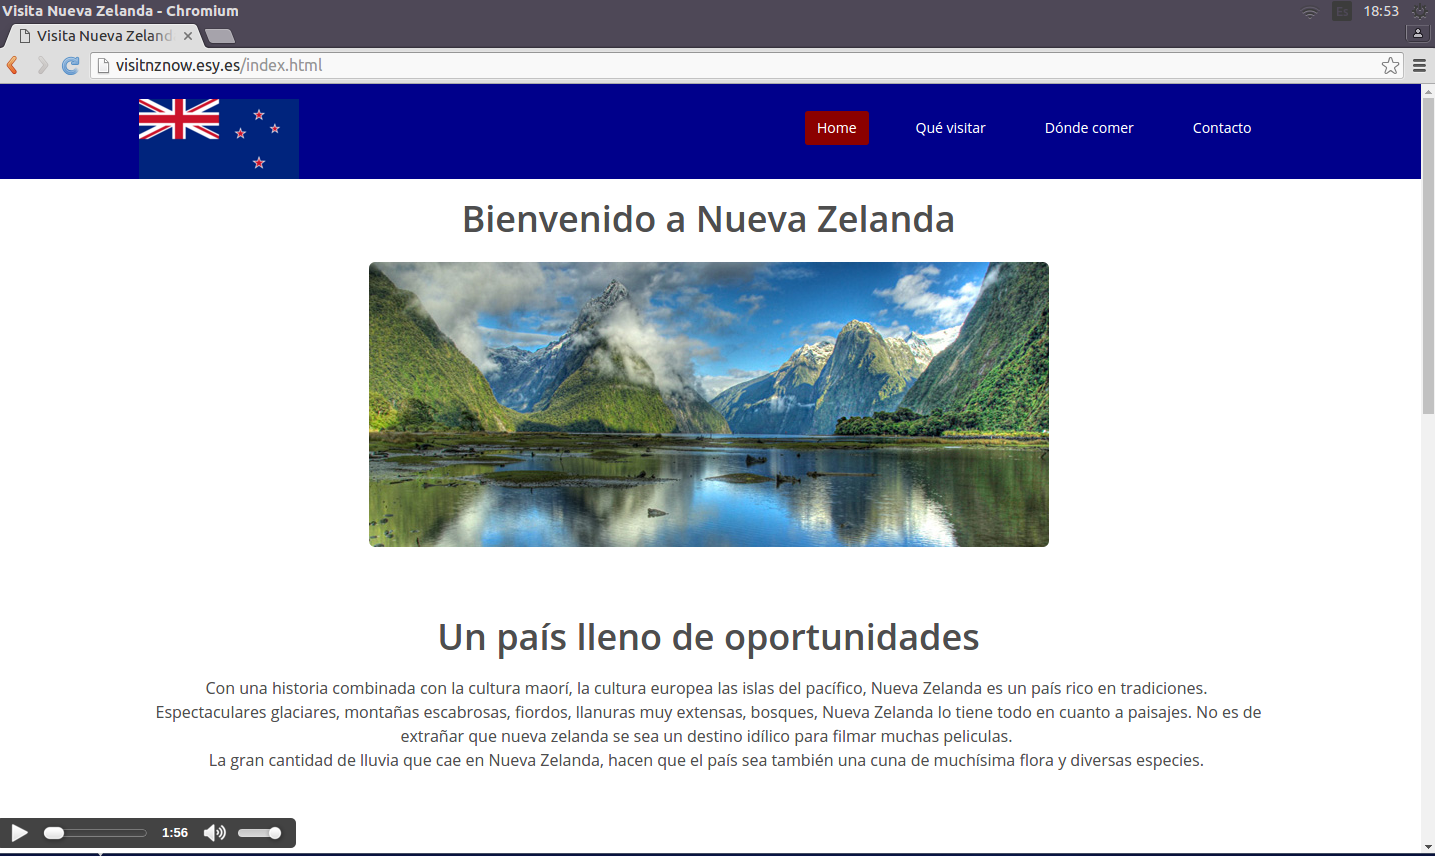
\includegraphics[width=0.95\textwidth]{./Fotos/chrome-capture.png}
	\caption{Captura de la página principal en Chrome}
	\label{fig: ejemplo}
\end{figure}
Como podemos observar, el aspecto es muy similar. El navegador necesitará tener instalado Adobe Flash Player para que se muestre la animación realizada en "animoto". \\ \\ También hay diferencias en el reproductor por defecto del navegador para el audio de nuestra página principal.

\subsubsection{Mozilla firefox}
\begin{figure}[h]
	\centering
	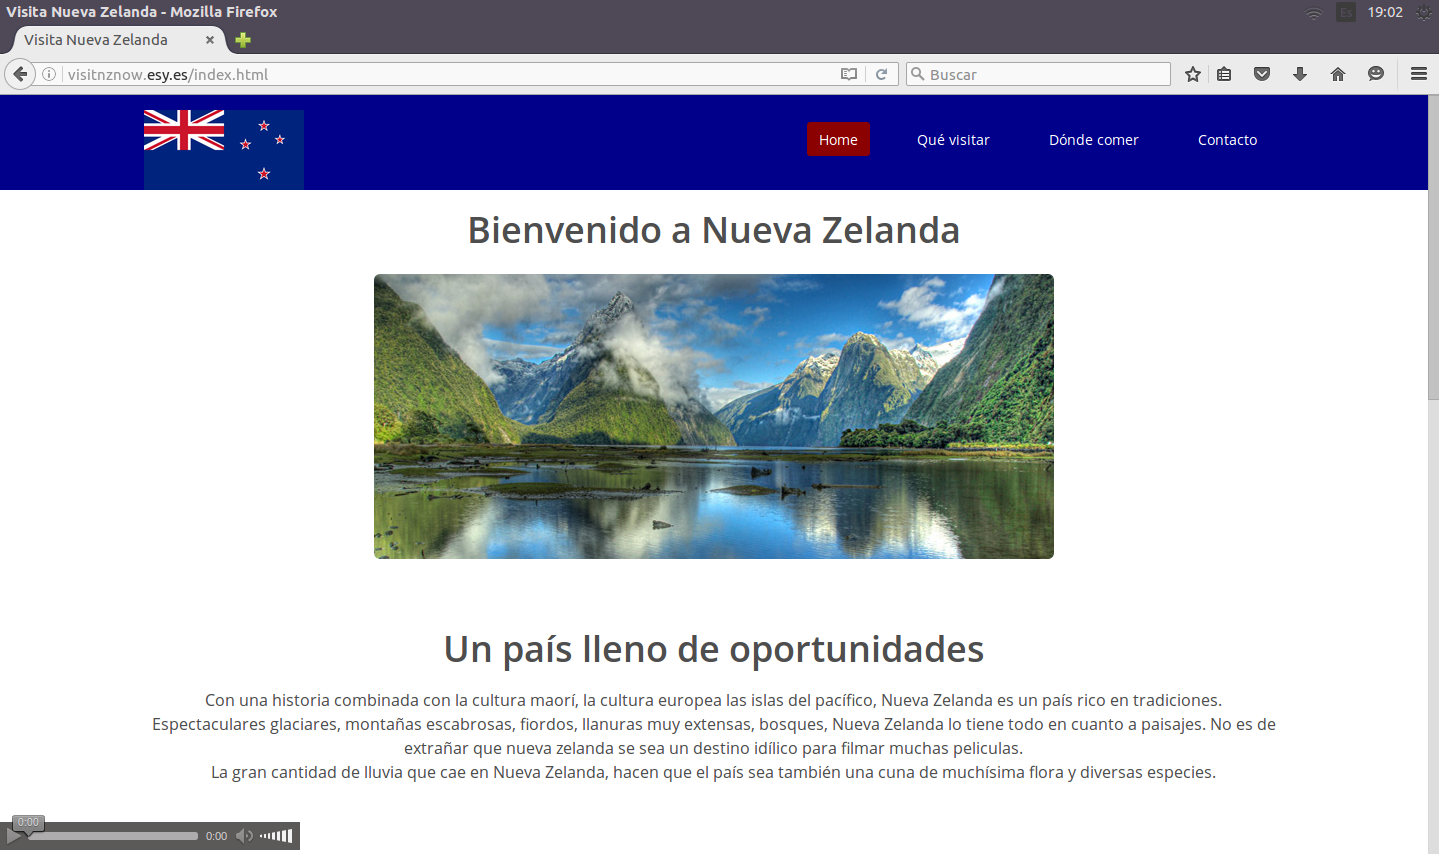
\includegraphics[width=0.95\textwidth]{./Fotos/firefox-capture.png}
	\caption{Captura de la página principal en firefox}
	\label{fig: ejemplo}
\end{figure}
Al igual que en chrome, es necesario instalar Adobe Flash player si no está instalado, para mostrar la animación. La apariencia del reproductor de audio cambia con respecto a Chrome.
\subsubsection{Internet explorer}
\subsubsection{Safari}
\subsubsection{Konkeror}
\subsection{Descripción de las principales dificultades}
\subsection{Conclusiones}
Tras realizar esta práctica nos hemos percatado de todos los puntos que hay que tener en cuenta a la hora de desarrollar una página con un buen nivel de accesibilidad. Aspectos como la navegación textual, el contraste o tamaño del texto, los efectos sonoros y visuales que a priori a nosotros no nos presentan ningún impedimento pueden convertirse en una barrera infranqueable para un determinado perfil de usuario.\\
Por ello todos estos puntos nos han hecho reflexionar sobre las diferentes capacidades que pueden tener los usuarios de nuestro software, así de la necesidad de tenerlos siempre en cuenta a la hora de desarrollar software.